\documentclass[useAMS,referee,usenatbib]{biom}
\usepackage{xcolor}
\usepackage{amsmath}
\usepackage{amsfonts}
\usepackage{amsmath}
\usepackage{graphicx}
\usepackage{multirow}
\usepackage{bbm}
\DeclareMathOperator{\E}{\mathbb{E}}
\newcommand{\vect}{\text{vec}}

\title[This is an Example of Recto Running Head]{Bayesian Functional Covariance Regression}

%  Here are examples of different configurations of author/affiliation
%  displays.  According to the Biometrics style, in some instances,
%  the convention is to have superscript *, **, etc footnotes to indicate 
%  which of multiple email addresses belong to which author.  In this case,
%  use the \email{ } command to produce the emails in the display.

%  In other cases, such as a single author or two authors from 
%  different institutions, there should be no footnoting.  Here, use
%  the \emailx{ } command instead. 

%  The examples below corrspond to almost every possible configuration
%  of authors and may be used as a guide.  For other configurations, consult
%  a recent issue of the the journal.

%  Single author -- USE \emailx{ } here so that no asterisk footnoting
%  for the email address will be produced.

%\author{John Author\emailx{email@address.edu} \\
%Department of Statistics, University of Warwick, Coventry CV4 7AL, U.K.}

%  Two authors from the same institution, with both emails -- use
%  \email{ } here to produce the asterisk footnoting for each email address

%\author{John Author$^{*}$\email{author@address.edu} and
%Kathy Authoress$^{**}$\email{email2@address.edu} \\
%Department of Statistics, University of Warwick, Coventry CV4 7AL, U.K.}

%  Exactly two authors from different institutions, with both emails  
%  USE \emailx{ } here so that no asterisk footnoting for the email address
%  is produced.

\author{John Shamshoian$^{1}$\email{donatello.telesca@ucla.edu}, Damla {\c S}ent{\"u}rk$^{1}$, Shafali Jeste$^{2}$, and Donatello Telesca$^{1,*}$ \\$^{1}$Department of Biostatistics, University of California, Los Angeles, California 90095, U.S.A.\\$^{2}$ Department of Psychiatry and Biobehavioral Sciences, University of California, Los Angeles,\\ California 90095, U.S.A.}
\title[Bayesian Functional Covariance Regression]{Bayesian Functional Covariance Regression}


\begin{document}


\label{firstpage}

%  put the summary for your paper here

\begin{abstract}
	% Case study type abstract
	%Many electroencephalography (EEG) studies aim to compare cognitive function between and within diagnostic groups. In our motivating study, resting state EEG data is collected on in a sample of 59 children with autism spectrum disorder and 38 age-matched typically developing (TD) controls. Peak alpha frequency (PAF), the frequency of maximal power within the alpha range (6 - 14 Hz), is a biomarker related to cognitive development and is known to increase with age in TD children. In this article we model alpha spectral power, rather than just the peak location. Patterns of variability of alpha spectral power between children are obscured by factors such as age. In the present work we develop methodology to estimate covariate-adjusted dependency patterns of alpha band oscillations, allowing for valid group level inference.  
	
	% More general abstract
	Function on scalar regression relates continuous outcomes to scalar predictors in expectation and finds many uses in applied domains such as medicine, public health, biomechanics, and environmental science. Equally important as the mean of the conditional mean function is the covariance operator, which has has relatively underdeveloped regression methods with some notable exceptions. In this article, we develop a Bayesian functional covariance regression model to provide full posterior inference to address this disparity. We also develop novel low-dimensional summaries which graphically indicate the degree of covariate-dependent heteroschedasticity. We apply our model to two motivating case studies to make novel insights. The first case study evaluates a functional biomarker of neural development in children with autism spectrum disorder and the second case study  explores the relationship between sleep patterns, age, and hypertension. 
\end{abstract}

%  Please place your key words in alphabetical order, separated
%  by semicolons, with the first letter of the first word capitalized,
%  and a period at the end of the list.
%

\begin{keywords}
	Autism spectrum disorder; Covariance regression; Functional data analysis; Peak alpha frequency; Power spectral density; Sleep heart health study.
\end{keywords}

%  As usual, the \maketitle command creates the title and author/affiliations
%  display 

\maketitle


\section{Introduction}
\label{s:intro}
\iffalse
The study investigated investigated peak alpha frequency (PAF), the frequency at which oscillations in the alpha rhythm [6-14 Hz] achieve maximal power and is known to shift from lower to higher frequencies as TD children age. The study found that children with ASD did not show increasing PAF with age. Furthermore, PAF was strongly correlated with non-verbal cognition. In this article we take a broader view and investigate the entire alpha spectrum as opposed to collapsing this information to a single point. EEG signals were recorded using a 128-channel sensor net at 500 Hz. After post-processing the raw EEG data, each child has 25 regions of interest and alpha spectral power captured from 6 to 14 Hz with .25 Hz increments. We propose to treat this data within a functional data framework, whree each spectral power curve is considered one observation. See \cite{Wang2016} for a broad review on functional data analysis (FDA). 
\fi

Functional data analysis (FDA) is a broad collection of theory and methods designed to analyze conceptually infinite-dimensional data with smoothness assumptions. Functional principal components analysis (FPCA) \citep{Wang2016} is ubiquitous in FDA, with applications ranging from biomedicine, gene expression data, environmental science, and many other scientific disciplines. Although the FPCA literature is growing rapidly to accommodate data arising from complex designs \citep{Baladandayuthapani2008, Staicu2010, Greven2010, Zipunnikov2011, Park2015, Scheffler2020}, only a handful of methods allow incorporating exogenous covariate information in the covariance estimation or resulting FPCA.  \cite{Cardot2007} developed a nonparametric technique based on kernel smoothers to smooth covariance surfaces over a covariate in dense functional data settings. \cite{Jiang2010} extended the kernel smoothing technique to accommodate sparse functional data by employing conditional expectation \citet{Yao2005}. \cite{Xiao2015} use sandwich smoothing \citep{Xiao2013} to extract age-adjusted patterns of variation in a repeated measures circadian rhythm study. \cite{Scheffler2020} extend the concept of weak-separability to incorporate exogenous covariate information in a multidimensional functional setting.

In this paper we develop a Bayesian procedure to adjust covariances based on exogenous covariate information. We focus on the independent functional response case for simplicity although extensions to more general dependency structures are possible. Our proposed method has three main contributions to the existing literature of covariate-adjusted covariance modelling:
\begin{itemize}
	\item \textbf{Straightforward inference.} The Bayesian paradigm offers a straightforward mechanism for uncertainty quantification. The alternative methods listed above must rely on the bootstrap. The literature surrounding bootstrapping in the presence of functional data is vague on handling many tuning parameters. Although there are some theoretical guarantees of the bootstrap in functional data settings \citep{Cuevas2006}, the literature is underdeveloped for models incorporating covariate information into the covariance function. In this paper we focus on uncertainty quantification for covariate-adjusted mean functions, covariate-adjusted covariance functions, and subject-specific latent trajectories.
	\item \textbf{Model-based.} Existing methods are based on highly flexible nonparametric techniques. However, users employing these methods must stratify their inferences by discrete covariates such as sex. In contrast, the proposed method accommodates discrete covariates in a single analysis due to the additive structure, retaining as much information as possible in the data without creating stratified analyses. 
	\item \textbf{Low-dimensional summaries.} We develop a low dimensional summary which aids in describing the amount of heterogeneity attributed to a particular covariate. It's not clear how to quantify this information using existing methods.
\end{itemize}

The proposed method is closely related to the notion of regularized covariance estimation. As an early reference for regularized covariance estimation, \citet{Flury1984} developed a method to estimate a common set of principal components across $k$ groups. This concept was generalized by \citet{Franks2019}, who use partial pooling to estimate a set of principal components across $k$ groups. \citet{Fox2015} developed a Bayesian nonparametric method for estimating a time-varying covariance matrix through factor matrix products, where the loading of the factor matrix depends on predictors. However it's unclear how to extend this method in the context of independent functional observations or include discrete covariates such as group indicators. Moreover, this particular method requires high dimensional Gibbs updates, which limits its computational feasibility. In contrast, the multivariate covariance regression model of \citet{Hoff2012} can incorporate continuous as well as discrete covariates and only requires low dimensional Gibbs updates. However, this flexibility is at the cost of some linear assumptions, making the method not as flexible as \citet{Fox2015} in some aspects. See \citet{Li2014} and \citet{Quintero2017} for extensions of this model to the multivariate multilevel case. The model presented in Section \ref{s:model} can be seen as a functional extension of \citet{Hoff2012} with some added flexibility, and we will highlight the similarities and differences as we go along. 

We apply the proposed method to two case studies. The first case study involves electroencephalography (EEG) brain signals recorded on children with autism spectrum disorder (ASD). ASD is a complex neurodevelopmental disorder that affects about 1 in 54 children. ASD is characterized by difficulty in communication, restricted repetitive behaviors, and stereotypical behavior. Low functioning children may have limited behavioral repertoire, necessitating specialized assessment methods.  Electroencephalography (EEG) provides a direct measure of postsynaptic brain activity and does not rely on behavioral output from young children with ASD, making EEG based biomarkers appealling for diagnosis, prognosis, and intervention purposes \citep*{Jeste2015}. In this study 59 heterogenous children with ASD and 38 age matched typically developing (TD) children had resting-state EEG signals recorded \citep*{Dickinson2017}. This study focused on oscillations in the alpha rhythm, which play a role in neural coordination and communication between distributed brain regions. We describe how random patterns of variation differ between children with ASD and their TD peers, providing novel insights into their neurodevelopmental differences.

The second case study analyzes EEG data collected as part of an in-home polysomnography for the Sleep Heart Health Study (SHHS). This large study was designed to identify factors for sleep-disordered breathing, such as age, blood pressure, or sleep patterns. In this article we simply quantify sleep as a functional response and explore how heteroschedasticity depends on age and hypertension status. Specifically, we quantify how random variations of delta spectral power change by age and hypertension status. 

The rest of this paper is organized as follows: Section \ref{s:model} gives the generating model for functional data, Section \ref{s:priors} lists prior choices and discusses the reasoning behind them, Section \ref{s:posteriors} briefly discusses computations involved for posterior calculations, Section \ref{s:simulation} gives a thorough simulation study assessing errors and coverage properties, Section \ref{s:data} showcases the model on the two motivating case studies, and Section \ref{s:discussion} concludes with a brief discussion. The sampling algorithm and additional simulation details are given in the supplement.

\section{Model}
\label{s:model}
In this section we present the model associating patterns of variability and time-stable covariates. Let $y_{i}(t)$ denote the outcome for subject $i$ at point $t \in \mathcal{T}$ for some real compact interval $\mathcal{T}$. Let $\bmath{x} = (x_{1},\ldots,x_{d_{1}})^{\top}$ denote a $d_{1}$-dimensional time-stable covariate for subject $i$, with the dependence on $i$ removed for ease of presentation. The $k$-dimensional data-generating model is 
\begin{gather}
y_{i}(t) = \mu(t, \bmath{x})   + r_{i}(t, \bmath{x})  + \epsilon_{i}(t)\label{eq:model}\\
r_{i}(t, \bmath{x}) = \sum_{j=1}^{k}\psi_{j}(t, \bmath{x})\eta_{ij}\label{eq:covariance}\\
\eta_{ij} \sim N(0, 1),\;\;\;\;\epsilon_{i}(t) \sim N(0, \varphi^{2})
\label{eq:random}
\end{gather}
where $\mu(t, \bmath{x})$ is the conditional mean, $\psi_{j}(t, \bmath{x})$ form conditional latent functional bases, $\eta_{ij} \sim N(0,1)$ are subject-specific scores, and $\epsilon_{i}(t) \sim N(0, \varphi^{2})$ represents measurement error. Using equations (\ref{eq:model}, \ref{eq:covariance}, \ref{eq:random}) the conditional covariance function $c(t, t', \bmath{x})$ is
\begin{gather}
c(t,t', \bmath{x}) = \sum_{j=1}^{k}\psi_{j}(t,\bmath{x})\psi_{j}(t',\bmath{x})\label{eq:covariance_form}
\end{gather}

We acknowledge that various approaches exist for specifying the form of $\mu(\cdot)$ and $\psi_{j}(\cdot)$ including local polynomial smoothers \citep{Fan1996}, kernel smoothers \citep{Ferraty2006}, Gaussian process methods \citep{Yang2016, Fox2015}, and spline procedures \citep{Ramsay2005}. Lending toward conceptually straight-forward prior assumptions, we  build $\mu(\cdot)$ and $\psi_{j}(\cdot)$ as linear combinations of spline bases. Borrowing notation from \citet{Scheipl2015}, $\mu(t, \bmath{x})$ can be written as
\begin{gather}
\mu(t, \bmath{x}) = \sum_{r=1}^{R}f_{r}(t, \bmath{x}_{r})
\end{gather}
where the set $\cup\{\bmath{x}_{r}\}_{r=1}^{R} = \bmath{x}$. This grouping framework leads to flexible specification of basis expansions. For example, when $\bmath{x}_{r}$ is a single scalar covariate $f_{r}(t, x_{r})$ could be a functional linear effect $x_{r}f(t)$ or a smooth effect $f(t, x_{r})$. If $\bmath{x}_{r} = (x_{r_{1}}, x_{r_{2}})$ is a vector of covariates, $f_{r}(t, \bmath{x}_{r})$ could be written as $f(t, x_{r_{1}}, x_{r_{2}})$,  $x_{r_{1}}f(t, x_{r_{2}})$, or $x_{r_{1}}x_{r_{2}}f(t)$. These terms are approximated by a set of basis functions with corresponding priors to encourage smooth effects. For the general case, we maintain that $\bmath{x}_{r}$ could be a vector with basis $\bmath{b}^{r}(\bmath{x}_{r}) = (b_{1}^{r}(\bmath{x}_{r}), \ldots, b_{p_{r}}^{r}(\bmath{x}_{r}))$. Then 
\begin{align}
f_{r}(t, x_{r}) &= \bmath{b}(t)^{\top}\beta_{r} \,\bmath{b}^{r}(\bmath{x}_{r})\label{eq:mu1}\\
\mu(t, \bmath{x}) &= \bmath{b}(t)^{\top} \beta \bmath{b}^{x}(\bmath{x}_{i})\label{eq:mu2}
\end{align}
where $\beta = \big(\beta_{1}\,|\cdots|\,\beta_{R}\big)$ and $\bmath{\tilde{X}}(\bmath{x}) = \big(\bmath{b}^{1}(\bmath{x}_{r})\,|\cdots|\,\bmath{b}^{R}(\bmath{x}_{r})\big)^{\top}$. Keeping track of dimensions,  $\beta$ is a $p\times r(d_{1})$ coefficient matrix and  $\bmath{b}^{x}(\bmath{x}_{i})$ is a $r(d_{1})\times 1$ vector, where $r(d_{1}) = \sum_{r=1}^{R}p_{r}$. We place another additive model on $\psi_{j}(t, \bmath{x})$. Namely, 
\begin{gather}\psi_{j}(t,\bmath{x}) = \sum_{r=1}^{R}l_{jr}(t,\bmath{x}_{r})\label{eq:psi_additivity}
\end{gather} where $l_{jr}$ are smooth effects in terms of $\bmath{x}_{r}$ for the $j$th conditional latent function basis function. Similar to $f_{r}(t,\bmath{x}_{r})$ and $\mu(t, \bmath{x})$, $l_{jr}(t, \bmath{x}_{r})$ and $\psi_{j}(t, \bmath{x})$ can also be written as products of matrices and vectors:
\begin{align*}
l_{jr}(t, x_{r}) &= \bmath{b}(t)^{\top}\Lambda_{jr} \,\bmath{b}^{r}(\bmath{x}_{r})\\
\psi_{j}(t, \bmath{x}) &= \bmath{b}(t)^{\top}\,\Lambda_{j} \bmath{b}^{x}(\bmath{x}_{i})
\end{align*} where $\Lambda_{jr}$ is a $p\times p_{r}$ loading matrix and  $\Lambda_{j} = \big(\Lambda_{j1}\,|\cdots|\,\Lambda_{jR}\big)$. The additivity on $\psi_{j}(t, \bmath{x})$ implies that the covariance function \ref{eq:covariance_form} is 
\begin{gather*}
c(t, t', \bmath{x}) = \sum_{j=1}^{k}\bigg(\sum_{r=1}^{R}\sum_{r'=1}^{R}l_{jr}(t,\bmath{x}_{r})l_{jr'}(t',\bmath{x}_{r'})\bigg)
\end{gather*} 
This convolution structure makes it difficult to define low dimensional summaries of covariate influence on the covariance function. Instead, we propose a low dimensional summary which quantifies the impact of a covariate on the  $l_{jr}$ functions directly. Let
\begin{equation}
g_{r}(t, \bmath{x}_{r}) = \sum_{j=1}^{k}l_{jr}(t,\bmath{x}_{r})^{2} \label{eq:low}
\end{equation}
summarize the effect of $\bmath{x}_{r}$ across $\psi_{j}$, $j=1,\ldots,k$. If the impact of $\bmath{x}_{r}$ on $\psi_{j}$, $j=1,\ldots,k$ is negligable, then $g_{r}(t, \bmath{x}_{r})$ will be near zero. Consequently if $g_{r}(t, \bmath{x}_{r})$ is near zero, the $c(t,t', \bmath{x})$ will not be sensitive to changes in $\bmath{x}_{r}$. To the best of our knowledge, this is the first attempt at quantifying the impact of covariates on a covariance function which is only possible through the additivity assumption on $\psi_{j}(t, \bmath{x})$ from equation \ref{eq:psi_additivity}.

Unlike previous work on functional covariance regression \citep{Cardot2007, Jiang2010}, equations (\ref{eq:model}, \ref{eq:covariance}, \ref{eq:random}) specify a generative model for functional covariance regression. Complete with priors detailed in Section \ref{s:priors}, posterior inference is evaluated through Markov-Chain Monte Carlo (MCMC). This is important because empirical methods require resampling to perform inference. However, resampling techniques for functional data come with pitfalls. Any fitted model will have smoothing bias (to regularize rapidly varying functions). A parametric bootstrap would generate data from a biased model, and subsequently cause even more bias by smoothing once again for each bootstrap replicate. Nonparametric bootstrapping causes undersmoothing due to the presence of repeated functions.

Outside of the FDA literature, \citet{Hoff2012} developed a similar model for covariance regression with multivariate data. However, as \citet{Fox2015} note, their mapping from predictors to covariance assumes a parametric form, thus limiting the model's expressivity. To overcome this parametric limitation, the authors develop a factor matrix process estimate a time-varying covariance matrix characterizing influenza incidence across the United States. This approach is flexible but each gibbs sample iteration requires a cholesky decomposition of an $n\times n$ matrix where $n$ is the number of subjects. The basis transform approach taken here would only require a cholesky decomposition of a $p \cdot r(d_{1}) \times p\cdot r(d_{1})$ matrix for each iteration. Therefore the basis transform approach is likely to scale better for large data sets such as the SHHS, provided $r(d_{1})$ is not too large.  
\section{Prior Distributions}
\label{s:priors}
In this section we place priors on all unknown quantities of interest. We begin by placing prior on $\mu(t, \bmath{x})$. As we have seen in equations \ref{eq:mu1} and \ref{eq:mu2}, this amounts to placing a prior on each $\beta_{r}$ submatrix. The rows of $\beta_{r}$ are associated with a $p\times p$ penalty matrix $K$, and the columns of $\beta_{r}$ are associated with a $p_{r}\times p_{r}$ penalty matrix $K_{r}$. These penalties are designed to encourage smoothness and can target magnitude penalization, squared derivative shrinkage, or local changes in $\beta_{r}$ through a differencing penalty. In this paper we penalize the second order difference of $\beta_{r}$ coefficients in both directions, but other penalties could be used as well. A prior for $\beta_{r}$ respecting the tensor structure is constructed as follows \citep{Wood2017}. Let $\tilde{K} = I_{p_{r}\times p_{r}}\otimes K$ and $\tilde{K_{r}} = K_{r} \otimes I_{p\times p}$. The prior for the vectorized form of $\beta_{r}$ is

\begin{gather*}
\vect(\beta_{r}) \,|\, \tau_{1xr}, \tau_{1tr} \sim\\ \exp\{-0.5\vect(\beta_{r})^{\top}( \tau_{1xr} \tilde{K}_{r} + \tau_{1tr}\tilde{K})\vect(\beta_{r})\}
\end{gather*} 
where $\tau_{1xr}, \tau_{1tr}$ are smoothing parameters. If $p_{r} = 1$ then $\beta_{r}$ is a $p\times 1$ vector and $\tilde{K}_{r} = 0$. In this case the prior simplifies to 
\begin{align*}
\beta_{r} \,|\tau_{1tr}\sim \exp\{-0.5\tau_{1tr}\beta_{r}^{\top}K\beta_{r}\}
\end{align*}
This prior is improper but provided that proper priors are set for $\tau_{1tr}, \tau_{1xr}$, the posterior of $\beta_{r}$ will be proper \citep{Lang2004}. Priors for $\psi_{j}(t, \bmath{x})$. However, $\psi_{j}(t,\bmath{x})$ for larger $j$ should also contribute less to the fit than earlier terms. Therefore the prior for $\psi_{j}(t,\bmath{x})$ should encourage smoothing and shrinkage aspects. Let $\Lambda_{rj}$ be the analogous component to $\beta_{r}$. Re-using the same penalty matrices as above, the prior for $\Lambda_{rj}$ is 
\begin{gather*}
\vect(\Lambda_{rj})\,|\,\tau_{2jxr},\tau_{2jtr}, \tau_{rj}^{*}, \phi_{rj} \sim \\\exp \{-0.5\vect(\Lambda_{rj})^{\top}(\tau_{2jxr}\tilde{K}_{r} + \tau_{2jtr}\tilde{K} + \tau^{*}_{rj}\phi_{rj})\vect(\Lambda_{rj})\}
\end{gather*}
where $\tau_{2jxr}, \tau_{2jtr}$ are smoothing parameters and $\phi_{rj}$, $\tau^{*}_{rj}$ are shrinkage parameters. Here $\phi_{rj}$ is a diagonal matrix with dimension $p\cdot p_{r}\times p\cdot p_{r}$. If $p_{r} =1$ (so that $\Lambda_{rj}$ is a column vector), then the prior becomes
\begin{gather*}
\Lambda_{rj} \,|\tau_{2jtr}, \tau^{*}_{rj},\phi_{rj} \sim\\
\exp\{-0.5\Lambda_{rj}^{\top}(\tau_{2jtr}\tilde{K} + \phi_{rj}\tau^{*}_{rj})\Lambda_{rj}\}
\end{gather*}
similar to the case when $\beta_{r}$ is a column vector. In summary, these priors for $\mu(t,\bmath{x})$ and $\psi_{j}(t,\bmath{x})$ are design to reflect our assumptions of smoothness in the functional data outcomes. All smoothing parameters are given a gamma prior distribution, 
\begin{gather*}
\tau_{1xr}, \tau_{1tr} \sim \text{Gamma}(a_{\tau}, b_{\tau})\\
\tau_{2jxr}, \tau_{2jtr} \sim \text{Gamma}(a_{\tau}, b_{\tau})
\end{gather*}
where we use the `rate' parameterization of the Gamma distribution (i.e., if $x \sim \text{Gamma}(a, b)$, then $\E[x] = a/b$). In addition we borrow the Gamma Multiplicative Process Prior (GMPP) from \cite{Bhattacharya2011, Montagna2012} to assign priors to $\tau^{*}_{rj}$ and $\phi_{rj}$. Let $\phi_{irj}$ denote the $i$th diagonal element of $\phi_{rj}$.
\begin{align}
\label{eq:phi}\phi_{irj}&\sim \text{Gamma}(a_{\phi}, b_{\phi})\\
\label{eq:shrink1}\tau^{*}_{rj} &= \prod_{l=1}^{r}\delta_{lr}\\
\label{eq:shrink2}\delta_{r1} &\sim \text{Gamma}(a_{r0}, 1)\\
\label{eq:shrink3}\delta_{rl} &\sim \text{Gamma}(a_{r1}, 1),\,\, l > 1\\
\label{eq:shrink4}a_{r0}, a_{r1} &\sim \text{Gamma}(2,1)
\end{align}
so that the $\tau_{rj}$ are stochastically increasing in $j$. This shrinkage is data-adaptive so that later entries of $\Lambda_{rj}$ may or may not be shrunk toward zero depending on the model fit. In particular, specifying a conservative choice of $k$ (number of latent functional factors) should not change results too much compared to setting $k$ to some ``optimal'' choice. 

\section{Posterior inference}
\label{s:posteriors}
We discuss posterior inference for subject-specific latent trajectories, mean functions, and principal directions of variation. In this paper we use the posterior mean as a point estimate and symmetric pointwise credible intervals for uncertainty quantification. Let $\hat{\beta}_{m}$, $\hat{\Lambda}_{jm}$, and $\hat{\eta}_{ijm}$ be the $m$th posterior draw of $\beta$, $\Lambda_{j}$, and $\eta_{ij}$. The point estimate for the $i$th subject-specific latent trajectory, $\tilde{y}_{i}(t)$, is $\frac{1}{M}\sum_{m=1}^{M}\{\bmath{b}(t)^{\top}\hat{\beta}_{m}\bmath{b}^{x}(\bmath{x}_{i}) + \sum_{j=1}^{k}\bmath{b}(t)^{\top}\hat{\Lambda}_{jm}\bmath{b}^{x}(\bmath{x}_{i})\}$. Similarly, the point estimate for the covariate-adjusted mean, $\mu(t, \bmath{x})$, is $\frac{1}{M}\sum_{m=1}^{M}\bmath{b}(t)\hat{\beta}_{m}\bmath{b}^{x}(\bmath{x}_{i})$. Let $C_{m}(\bmath{x})$ be the matrix given by evaluating the $m$th posterior draw of $c(t,t', \bmath{x})$ on a subset of $\mathcal{T}\times \mathcal{T}$. Performing a spectral decomposition on $C_{m}(\bmath{x})$ yields the $m$th draw of ordered orthonormal posterior principal directions of variation (eigenfunctions) $\tilde{\psi}_{jm}(t, \bmath{x})$, $j = 1,\ldots, k$. However, this method can be computational expensive due to the spectral decomposition of arbitrarily high-dimensional matrix $C_{m}(\bmath{x})$ due to the nature of functional data. To alleviate this burden, we follow  \cite{Aguilera2013} and only perform a spectral decomposition on a low-dimensional matrix, $\sum_{j=1}^{k}\hat{\Lambda}_{jm}\bmath{b}^{x}(\bmath{x}_{i})\bmath{b}^{x}(\bmath{x}_{i})^{\top}\hat{\Lambda}_{jm}^{\top}$, so that we never actually form $C_{m}(\bmath{x})$ in our implementation. Since $\tilde{\psi}_{jm}(t, \bmath{x})$ is only identifiable up to sign change, each $\psi_{jm}(t, \bmath{x})$ may be potentially multiplied by $-1$ to orient all eigenfunctions correctly. More details on extracting and orienting posterior eigenfunctions are provided in Web Appendix D. Once all posterior eigenfunctions are oriented correctly, a point-estimate is obtained by simply taking the posterior pointwise mean. 

Credible intervals are computed in the following manner. Let $\mu_{f}(t)$ and $\sigma_{f}(t)$ be the posterior mean and standard deviation of some functional $f(\cdot)$ evaluated at $t$. A $(1-\alpha)\cdot 100$ credible interval for $f(t)$ is $[\hat{f}(t) - z^{*}_{1-\alpha/2}\sigma_{f}(t), \hat{f}(t) + z^{*}_{1-\alpha/2}\sigma_{f}(t)]$ where $z^{*}_{1-\alpha/2}$ is the $1-\alpha/2$ quantile of the standard normal distribution. Pointwise intervals have nominal average coverage when the model is correctly calibrated. However, pointwise intervals are anti-conservative when performing inference for an entire function $f(\cdot)$. In this case we recommend computing simultaneous credbile bands. Our implementation includes this option and we give more details in Web Appendix B.




\section{Simulations}
\label{s:simulation}
\iffalse Analytic posterior distributions are intractable, so we rely on Markov-Chain Monte-Carlo techniques to draw samples from all relevant posterior distributions. Since all full conditionals of blocks of parameters are available in closed form, a simple Gibbs sampler updates each parameter block sequentially. See Web Appendix A for all block parameter updating steps.

%When the target of inference is a function $f$, as opposed to a single point, we adopt methodology from \citet{Crainiceanu2007} to form simultaneous credible bands. Suppose the domain of $f$ is $[t_{1}, t_{N}]$ and let $t_{1} < \ldots < t_{N}$ be a fine grid of points on this interval. Let $\mathbb{E}\{f(t_{j})\}$ and $\text{SD}\{f(t_{j})\}$ be the pointwise posterior mean and standard deviation of $f(t_{j})$ respectively. Let $\alpha^{*}$ be the $(1-\alpha)$ sample quantile of $\max_{1\leq j \leq N} |f(t_{j}) - \mathbb{E}\{f(t_{j})\}|/\text{SD}\{f(t_{j})\}$. Then $\mathbb{E}\{f(t_{j})\} \pm \alpha^{*} \text{SD}\{f(t_{j})\}, 1\leq j\leq N$ constitute $(1-\alpha)$ simultaneous credible intervals. This simultaneous credible band will be used to evaluate uncertainty in the mean and aspects of the covariance in Section~\ref{s:data}.

\fi 
We assess the performance of the proposed method in terms of mean, covariance, and latent response point estimation and coverage. We generate data under two scenarios. The first scenario has heteroscedasticity depending on a covariate $x$ scaled within the unit interval, and the second scenario imposes no such relationship between heteroscedasticity and covariates. Both scenarios include a covariate-dependent mean surface. We fit data generated in both scenarios by (1) the proposed method, adjusting for covariate-dependent heteroscedasticity and (2) foregoing this adjustment and assuming the covariate only impacts the mean structure. We generate data in both scenarios by simulating from the model. We generate 300 datasets per scenario and true model parameters are kept fixed over each dataset. We include two sample sizes $N=100$ and $N=400$ to numerically verify mean and covariance point estimation convergence. 

We begin by using a p-spline of dimension 10 to expand the functional arguement $t$ and a p-spline of dimension 5 (not including an intercept) to expand the covariate argument $x$. According to notation from section \ref{s:model}, $\bmath{b}(t) = (b_{1}(t), \ldots, b_{10}(t))^{\top}$, $\bmath{b}^{2}(x) = (b_{1}^{2}(t),\ldots,b_{5}^{2}(t))^{\top}$,  and $\mu(t, x) = f_{1}(t) + f_{2}(t, x) = \bmath{b}(t)\,\beta_{1} + \bmath{b}(t)\,\beta_{2}\,\bmath{b}^{2}(x)$. The model parameters $\beta_{1}$ and $\vect(\beta_{2})$ have prior mean zero and precision $\Omega_{1} + \epsilon\cdot I_{10\times10}$ and $\Omega_{2} + \epsilon\cdot I_{50\times50}$ respectively. The nugget term $\epsilon\cdot I$ is used to simulate from a full-rank multivariate normal and in our experiments we set $\epsilon = .1$. To ensure smoothness of the resulting response functions $y_{i}(t)$, we set $\Omega_{1} = \tau_{1t1}K$ and $\Omega_{2} = \tau_{1x2}(K_{2}\otimes I_{10\times 10}) + \tau_{1t2}(I_{6\times 6}\otimes K)$, where $K$ and $K_{2}$ are second order discrete penalty matrices associated with p-splines. We use $k = 4$ latent functional factors for the random component $r_{i}(t, x)$, so $r_{i}(t, x) = \sum_{j=1}^{4}\psi_{j}(t, x)$. Under data-generating scenario 1, we set $\psi_{j}(t, x) = l_{j1}(t) + l_{j2}(t, x)$. Under data-generating scenario 2, we set $\psi_{j}(t, x) = l_{j1}(t)$. Expanding out the terms, $l_{j1}(t) = \bmath{b}(t)^{\top}\,\Lambda_{j1}$ and $l_{j2}(t, x) = \bmath{b}(t)\,\Lambda_{j2}\,\bmath{b}^{2}(x)$. The model parameters $\Lambda_{j1}$ and $\Lambda_{j2}$ prior mean zero and prior precision $\Gamma_{j1}$ and $\Gamma_{j2}$ respectively. We set $\Gamma_{j1} = \tau_{2t1}K + \tau^{*}_{1j}$ and $\Gamma_{j2} = \tau_{2x2}(K_{2}\otimes I_{10\times 10}) + \tau_{2t2}(I_{6\times 6}\otimes K) + \tau_{2j}^{*}$. Smoothing and shrinkage parameters are  $\tau_{1t1} = \tau_{1t2} = \tau_{2t1} = \tau_{2t2} = 10$, $\tau_{1x2} = \tau_{2x2} = 100$, $\tau^{*}_{1j} = 2^{j}$, and $\tau^{*}_{2j} = 4^{j}$. Measurement error is $\varphi^{2} = .20^{2}$ and functional data $y_{i}(t)$ is generated according to equation \ref{eq:model}. The functional argument $t$ is evaluated at 100 equally spaced locations within the unit interval and $x_{i}$ is equal to $(i - 1) / (N-1)$. 

It will be convenient to divide data-generating scenarios and fitting procedures into four separate cases. Case 1 has data generated from scenario 1, fit with a model that adjusts for heteroscedasticity due to the covariate. Case 2 has data generated from scenario 2, fit with a model that does not adjust for heteroscedasticity due to the covariate. Case 3 has data generated from scenario 2, fit with a model that adjusts for heteroscedasticity due to the covariate. Case 4 has data generated from scenario 2, fit with a model that does not adjust for heteroscedasticity due to the covariate. We fit each dataset with with $k = 6$ latent functional factors and expand the functional argument into a p-spline basis of dimension 10. We expand the covariate argument into a p-spline basis of dimension 7. In doing so, we simply enlarge the model space and test its ability to regularize unnecessary latent dimensions and basis expansions. We place uniform priors on all smoothing parameters and a $\text{Gamma}(0.0001, 0.0001)$ prior on the inverse measurement error, $\varphi^{-2}$. We fit each model with 50,000 samples, discarding 25,000 as burn-in and keeping every 5th observation to save computer memory. We keep track of coverage, average credible interval width, and relative integrated squared error (RISE). The coverage performance assess a model's calibration and goodness of fit, whereas RISE assesses a model's performance in terms of point estimation. 

Let $t_{1}, \ldots, t_{100}$ be 100 uniformly placed points along the domain of the functional argument, $x^{*}_{1},\ldots,x^{*}_{10}$ be uniformly placed points along the interval $[0.1, 0.9]$, and $\tilde{y}_{i}(t)$ denote the latent response of $y_{i}(t)$ uncontaminated with random error. Let $\mathbbm{1}(\cdot)$ be the indicator function that returns 1 when the argument is true and 0 otherwise. The coverage of $\mu(t, x)$ is $\frac{1}{1000}\sum_{i=1}^{10}\sum_{m=1}^{100}\mathbbm{1}\{\mu(t_{m}, x^{*}_{i}) \in \widehat{I}_{mi}\}$, the coverage of $c(t, t', x)$ is $\frac{1}{50500}\sum_{i=1}^{10}\sum_{m=1}^{100}\sum_{m'=1}^{m}\mathbbm{1}\{c(t_{m},t_{m'},x^{*}_{i})\in \widehat{I}_{mm'i}\}$, and the coverage of $\tilde{y}_{i}(t)$ is $\frac{1}{N\times 100}\sum_{i=1}^{N}\sum_{m=1}^{100}\mathbbm{1}\{\tilde{y}_{i}(t_{m}) \in \widehat{I}_{y,mi}\}$, where $\widehat{I}_{mi}$ is the nominal 95\% posterior interval about $\mu(t_{m}, x_{i})$ and $\widehat{I}_{mm'i}$ is the nominal 95\% posterior interval about $c(t_{m},t_{m'}, x_{i})$, and $\widehat{I}_{y,mi}$ is the nominal 95\% posterior interval about $\tilde{y}_{i}(t)$. The RISE of $\mu(t, x)$ is $100\cdot\frac{\sum_{i=1}^{10}\int_{\mathcal{T}}\,\{\widehat{\mu}(t, x^{*}_{i}) - \mu(t, x_{i}^{*})\}^{2}\,dt}{\sum_{i=1}^{10}\int_{\mathcal{T}}\mu(t, x_{i}^{*})^{2}\,dt}$, the RISE of $c(t, t', x)$ is $100 \cdot  \frac{\sum_{i=1}^{10}\int_{\mathcal{T}}\int_{\mathcal{T}}\{\widehat{c}(t,t', x_{i}^{*})-c(t,t',x_{i}^{*})\}^{2}\,dt\,dt'}{\int_{\mathcal{T}}\int_{\mathcal{T}}\sum_{i=1}^{10}c(t,t',x_{i}^{*})^{2}\,dt\,dt'}$, and the RISE of $\tilde{y}_{i}(t)$ is $100\cdot \frac{\sum_{i=1}^{N}\int_{\mathcal{T}}\{\widehat{y}_{i}(t)-\tilde{y}_{i}(t)\}^{2}\,dt}{\sum_{i=1}^{N}\int_{\mathcal{T}}\tilde{y}_{i}(t)^{2}\,dt}$. In practice we use the trapezoidal rule to evaluate all integrals. We also compute average credible band width for $\mu(t, x)$, $c(t, t', x)$ and $\tilde{y}_{i}(t)$. All coverage, RISE, and interval width results are reported in Table \ref{t:simulation}.

We observe at least 95\% coverage for both $\mu(t, x)$ and $\tilde{y}_{i}(t)$ under all four cases. Adjusting for covariate-dependent heteroscedasticity does not seem to affect the coverage rates for $\mu(t, x)$ and $\tilde{y}_{i}(t)$. Coverage rates for $c(t, t', x)$ are slightly below the nominal 95\% in case 1, indicating that inference on $c(t, t', x)$ may be anti-conservative under covariate-dependent heteroschedasticity. As expected, coverage rates are low for $c(t, t', x)$ under case 2, where the data-generating truth has covariate-dependent heteroscedasticity but the model does not account for this. The coverage rate gets smaller from $N=100$ to $N=400$ samples due to tighter credible bands. We also see that adjusting for covariate-dependent heteroscedasticity does not alter the width of credible intervals by a substantial amount when the data-generating truth has no covariate-dependent heteroscedasticity. 

We notice slightly greater RISE for $\mu(t, x)$ and $\tilde{y}_{i}(t)$ in case 2 compared to case 1, indicating that adjusting for covariate-depending heteroscedasticity can lead to efficiency gains in estimating the mean structure, even with only $N=100$ samples and only modest covariate-dependent heteroscedasticity. Estimation error for $\mu(t, x)$ and $\tilde{y}_{i}(t)$ is about the same under cases 3 and 4, indicating not much evidence of efficiency loss when the proposed adjustment is not necessary. However, the covariance estimation error is larger for case 3 than case 4, which indicates that the covariate-dependent heteroscedasticity adjustment can lead to slightly larger estimation error in the covariance structure when this adjustment is not necessary. 

Overall, the simulation shows that the proposed method can lead to gains in estimation and coverage (compared to a homoscedastic model) when the data has covariate-dependent heteroscedasticity. Cases 3 and 4 show that estimation error for the mean structure is robust to choice of model under a homoscedastic data-generating mechanism. However, making this adjustment under a homoschedastic data-generating mechanism leads to slightly larger estimation error in the covariance structure. We recommend exploring values of $g(t, x)$ to decide whether or not to adjust the variance by covariates. 
\begin{table}
	\caption{Simulation results over 300 data sets for each sample size and case combination. Coverage, error (RISE), and interval width are averaged over all data sets. Refer to Section \ref{s:simulation} for details on how coverage, error, and interval width are calculated.}
	\label{t:simulation}
	\begin{center}
		\begin{tabular}{lllccc}
			\Hline
			 Sample size & Quantity &Case & Coverage&  Error &  Interval width\\ \hline
			\multirow{12}{*}{$N=100$} & \multirow{4}{*}{$\mu(t,x)$}  & 1 &  .98&  .84& .30 \\
			&& 2 & .98& .91& .32 \\
			&& 3 & .98& .78& .30\\
			&& 4 & .98& .79& .30\\
			\cline{2-6}
			&\multirow{4}{*}{$c(t,t',x)$} & 1 & .89& 7.00& .14\\
			&& 2 &.72&9.76&.11\\
			&& 3 &.98&4.31&.13\\
			&& 4 &.97&3.29&.11\\
			\cline{2-6}
			&\multirow{4}{*}{$y_{i}(t)$} & 1 & .97& .25& .17\\
			&& 2 &.97&.29&.19\\
			&& 3 &.98&.21&.17\\
			&& 4 &.98&.20&.16\\
			\hline
			\multirow{12}{*}{$N=400$} & \multirow{4}{*}{$\mu(t,x)$}  & 1 &.99 & .19& .18 \\
			&& 2 & .98& .21& .19 \\
			&& 3 &.99 & .18& .18 \\
			&& 4 &.98 & .18& .18\\
			\cline{2-6}
			&\multirow{4}{*}{$c(t,t',x)$} & 1 & .88 & 3.10& .09\\
			&& 2 & .46&7.23&.06\\
			&& 3 &.98&1.01&.06\\
			&& 4 &.97&.84&.05\\
			\cline{2-6}
			&\multirow{4}{*}{$y_{i}(t)$} & 1 &.97 & .13 &.16 \\
			&& 2 &.97&.18&.18\\
			&& 3 &.98&.12&.16\\
			&& 4 &.98&.12&.16\\
		\end{tabular}
	\end{center}
\end{table}

\section{Case Studies}
\label{s:data}
\subsection{Application to ASD study}
Peak alpha frequency (PAF), the frequency at which oscillations in the alpha range demonstrate maximal power, shows well-characterised increases with chronological age during childhood in typically developing children \citep{Somsen1997, Dustman1999, Stroganova1999, Chiang2011, Cragg2011, Miskovic2015}. PAF has been shown to index neural development in TD children \citep{Valdes2010, Segalowitz2010, Rodriguez2017}. However, a recent study by \citet{Dickinson2017} found that children with ASD did not show the typical increase in PAF with age. In the present study, we investigate the relationship between diagnostic status, age, and alpha spectral density. Treating alpha spectral density as a functional response avoids complicated PAF identification procedures \citet{Dickinson2017} and retains more information as opposed to collapsing the entire alpha spectral band to a single point \citep{Scheffler2019, Scheffler2020}. In this study we wish to characterize functional mean and covariance dependence of alpha spectral density in terms of age and diagnostic status. 

In the \citet{Dickinson2017} study, resting-state EEG was collected on 39 TD children and 58 children with ASD aged 2 to 12 years old.  EEG signals were sampled at 500 Hz for two minutes and interpolated to a 10-20 25 channel montage \citep{Jasper1958, Perrin1989}. Alpha spectral density  $\Omega \in [6 \text{ Hz}, 14 \text{ Hz}]$ were obtained for each electrode. To facilitate comparisons across regions and subjects, alpha spectral density was normalized to unit area. See \cite{Scheffler2019} for more details on data acquisition and pre-processing. The resulting data structure is region-referenced functional data, which induces correlated responses within subjects. Unfortunately, the proposed method can not accommodate correlated functional data. Instead, for demonstration purposes, we only examine one region at a time. We also acknowledge that \citet{Scheffler2020} already successfully applied a covariate-adjusted hybrid principal components analysis, which can accommodate correlated functional responses within subject. While the goals of \citet{Scheffler2020} are similar to the ones posed in this article, we note that this method is (1) based on a Bayesian method, which yields stochastic regularization and straight-forward inference and (2) the low dimensional summary in eq. \ref{eq:low} provides some insight into how the variability of normalized alpha spectral density as a function of age and diagnostic status. 

We treat normalized alpha spectral density from the T8 region as the functional response and adjust the mean and covariance functions by diagnostic status, age, and a diagnostic status by age interaction. This interaction is scientifically motivated because as previously mentioned, PAF increases with age for TD children but not so for children with ASD. For the frequency dimension, we use a p-spline basis with 12 degrees of freedom using a second order differencing penalty. We expand age via p-splines with 6 degrees of freedom, again with a second order difference penalty. We run a markov chain monte carlo algorithm for 200,000 iterations. To save on memory purposes, we only save every 20 iterations. Of the leftover 10,000 iterations, we discard the first 5,000 as burn-in and keep the subsequent 5,000 for inference.  

Figure \ref{fig:asd_means} plots normalized alpha spectral density over several ages of child and diagnostic group with associated 95\% pointwise credible bands. The means curves drift apart as the cross-sectional age increases, which supports the notion that differences in alpha spectral band dynamics between ASD and TD children at similar ages can successfully predict diagnostic status \cite{Scheffler2019}. 

Furthermore, we explore age and group adjusted patterns of variability. Figure \ref{fig:asd_eigen1} displays the leading age and group adjusted eigenfunction. The general shape for a particular age is a unimodal curve peaked around 8-10 Hz. Notice that the peak of this curve tends to shift from lower to higher frequencies as age increases for the TD group, whereas the peak frequency is relatively constant over age for the ASD group. This finding was previously discovered by \cite{Scheffler2020} who estimate covariate-adjusted eigenfunctions in a similar to the proposed method but also account for the regional dimension. On the other hand, posterior summaries $g(t, \bmath{x})$ in Figure \ref{fig:asd_g} indicate that most variability is due to group as opposed age.

\begin{figure}
	\centering
	\includegraphics[width=1\textwidth]{/Users/johnshamshoian/Documents/R_projects/bfcr/Peak Alpha Data/Graphics/means.pdf}
	\label{fig:asd_means}
	\caption{Posterior mean alpha spectral power for ASD and TD groups at age 50, 70, 90, and 110 months.}
\end{figure}
\begin{figure}
	\centering
	\includegraphics[width = .8\textwidth]{/Users/johnshamshoian/Documents/R_projects/bfcr/Peak Alpha Data/Graphics/eigen1.png}
	\label{fig:asd_eigen1}
	\caption{Posterior mean of first leading covariate-adjusted eigensurfaces.}
\end{figure}
\begin{figure}
	\centering
	\includegraphics[width = .6\textwidth]{/Users/johnshamshoian/Documents/R_projects/bfcr/Peak Alpha Data/Graphics/covariate_effects_parsed.pdf}
	\label{fig:asd_g}
\end{figure}

\subsection{Application to Sleep Heart Health Study}
The Sleep Heart Health Study (SHHS) was a prospective cohort study designed to investigate obstructive sleep apnea (OSA) and other sleep-disordered breathing (SDB) as risk factors for the development of cardiovascular disease \citep{Quan1997}. Parent cohort studies and recruitment targets for these cohorts are the following: Atherosclerosis Risk in Communities Study (1,750 participants), Cardiovascular Health Study (1,350 participants), Framingham Heart Study (1,000 participants), Strong Heart Study (600 participants), New York Hy- pertension Cohorts (1,000 participants), and Tucson Epidemiologic Study of Airways Obstructive Diseases and the Health and Environment Study (900 participants). An unattended in-home polysomnography was completed by participants between November 1, 1995 and January 31, 1998. Between January 2001 and June 2003, a second polysomnogram was obtained in 3295 of the participants. %The baseline SHHS cohort included 52.9\% women and 47.1\% men. The race distribution was 81\% Caucasians, 9.\% Native-Americans, 8.0\% African-Americans, 1.3\% Asians, and 0.03\% `other' race category. The minimum age of enrollment was 40 years and there was no upper limit. The mean age was 62.9 (SD 11.0) years old. 

The American Academy of Sleep recognizes four sleep stages: stage N1 (light sleep), stage N2 (relaxation), stage N3 (slow-wave sleep), and stage R (rapid-eye movement). Importantly, N3 sleep, or slow-wave sleep (SWS) consists of high amplitude ($\geq$ 75 $\mu$V) and low-frequency  $(0.5-4.0)$ delta waves. SWS is considered to be most restorative sleep stage and to be associated with sleep quality, sleep maintenance, and functions toward memory consolidation \citep{Bonnet1987, Akerstedt1997, Walker2009}. \citet{Mander2017} reports that advancing into the fifth decade of age comes with (1) reduced SWS time and (2) increased time spent in lighter sleep stages (N1, N2). In addition, \citet{Javaheri2018} reports that lower levels of percent SWS sleep are associated with increased odds of incident hypertension in both men and women, independent of confounders such as sleep apnea, age, and sex. Most clinical studies (including the papers referenced above) quantify sleep by classifying time-varying electrical phenoma into discrete sleep stages. Subsequently, amount of SWS is represented by a single number, which is commonly percentage of sleep time in stage N3. However, this approach comes with several limitations \citep{Crainiceanu2009} including low intraclass correlation coefficient, no biological basis, and loss of temporal information. In this paper follow \citet{Crainiceanu2009, Di2009} and use power spectral density analysis to quantify sleep EEG. Our present goal is to characterize age-related changes in sleep between hypertension and non-hypertension groups. 

We use the discrete fast Fourier transform to analyze the sleep EEG data in the frequency domain. The entire night of sleep is broken into 30-second adjacent sleep epochs to account for temporal effects. These 30-second windows are processed using Welch's method of 50\% overlapping windows (4 second windows with 2 seconds overlap), where the intervals are windowed using a tapered Tukey window. The epoch-level power spectral density estimate is the average of the windowed power spectra. We use a band-pass filter to attenuate signals less than .3 Hz and greater than 35 Hz with a .5 Hz transition width. We mask epochs where artifacts detected using the method described in \citet{Buckelmuller2006}. We also mask epochs that are statistical outliers using (2, 2) Hjorth parameters \citet{Hjorth1970}. We compute delta spectral power by summing power spectra from 0.5 Hz to 4.0 Hz in .25 Hz increments on an epoch-by-epoch basis. To facilitate comparisons across participants, we compute epoch-level relative delta power spectral density (RDPSD) by dividing this power density by a summation of spectral density from .5 Hz to 35 Hz in .25 Hz increments. All filtering and power spectral density computations were performed in Luna \citep{Shaun2020}, which is an open-source software package for manipulating and analyzing polysomnographic readings.

We restrict our attention to EEG data collected on the first visit. We also filter participants to only include those who scored at least four hours of artifact-free signal. We analyze the first two hours of sleep, resulting in a dense grid of length 240 epochs for each participant. The 10th and 90th percentiles of age are 47 and 77 years-old, respectively. There are 2177 participants with hypertension and 3081 participants without hypertension. We use a p-spline of dimension 24 for the marginal basis for epoch and a p-spline of dimension 8 for the marginal basis for age. Each basis is associated with a second order differencing penalty matrix. We also include a hypertension dummy variable and a hypertension-age interaction. Exploratory analysis from \citet{Castro1986, fdapace} shows 9 principal components are needed to explain 99\% of variability (unadjusted for age and hypertension group). We fit our model with $k = 12$ latent factors since unneeded latent factors will be set close to zero due to the prior shrinkage process in equations \ref{eq:shrink1}-\ref{eq:shrink4}. We ran the MCMC algorithm described in the supplement for 200,000 iterations with a burn-in of 100,000, saving every 20th iteration for memory requirements.   

Figure \ref{fig:sleep_mean} displays mean RDPSD with associated 95\% point-wise credible intervals for ages 50, 60, 70, and years old for both hyertension and non-hypertension groups. Relative power spectral density decreases in N3 (around epoch 60) with age for both groups. The seemingly little decrease of SWS from midlife to late life is supported by \cite{Van2000}, who found that percent SWS predominantly decreases from early adulthood to midlife, with no further decrease into late life. Their study included 149 healthy men aged 16 to 83 years. Our methods support their finding after considering a much richer metric than percent SWS in the context of a much larger observational study. There is considerable overlap in the credible intervals between the hypertension and non-hypertension RDPSD, which does not support the hypothesis that hypertension is associated with increased levels of RDPSD. 


\begin{figure}
	\centering
	\includegraphics[width=1\textwidth]{/Users/johnshamshoian/Documents/R_projects/bfcr/sleep/Graphics/means.pdf}
	\label{fig:sleep_mean}
\end{figure}
We conducted an eigen-analysis on the model-based covariance surfaces. The estimated leading eigenfunction for a 50 year old with no hypertension accounts for 31\% of total variability and is positive over the entire epoch grid, suggesting that this component represents an overall RDPSD size construct. This eigenfunction, nor subsequent eigenfunctions vary much over age or group. The intercept effect is of $g(t, \bmath{x}_{r})$ is very large compared to age, group, and interaction effects, which means that between-subject heteroscedasticity does not depend much on these covariates. RDPSD is a heteroscedastic-stable metric when accounting for age and hypertension.

\begin{figure}
	\centering
	\includegraphics[width = .8\textwidth]{/Users/johnshamshoian/Documents/R_projects/bfcr/sleep/Graphics/eigen1.png}
\end{figure}
\begin{figure}
	\centering
	\includegraphics[width = .6\textwidth]{/Users/johnshamshoian/Documents/R_projects/bfcr/sleep/Graphics/covariate_effects_parsed.pdf}
\end{figure}

\section{Discussion}
\label{s:discussion}

We developed a probabilistic model suitable for functional data with covariate-dependent heteroscedasticity. The proposed apprach is computationally feasible for moderately large datasets such as the sleep study, which has $N = 5258$ subjects, 240 timepoints, and 16 basis functions for the covariate dimension. This feasibility is owed to tractible lower dimensional gibbs sampling updates. We also engineer low dimensional summaries of covariate-dependent heteroschedasticity, which can be used in practice to graphically aid in deciding whether to use a simpler model. 

%  The \backmatter command formats the subsequent headings so that they
%  are in the journal style.  Please keep this command in your document
%  in this position, right after the final section of the main part of 
%  the paper and right before the Acknowledgements, Supporting Information (Supplementary %  Materials),   and References sections. 

\backmatter

%  This section is optional.  Here is where you will want to cite
%  grants, people who helped with the paper, etc.  But keep it short!

\section*{Acknowledgements}

%The authors thank Professor A. Sen for some helpful suggestions, Dr C. R. Rangarajan for a critical reading of the original version of the paper, and an anonymous referee for very useful comments that improved the presentation of the paper.\vspace*{-8pt}



%  Here, we create the bibliographic entries manually, following the
%  journal style.  If you use this method or use natbib, PLEASE PAY
%  CAREFUL ATTENTION TO THE BIBLIOGRAPHIC STYLE IN A RECENT ISSUE OF
%  THE JOURNAL AND FOLLOW IT!  Failure to follow stylistic conventions
%  just lengthens the time spend copyediting your paper and hence its
%  position in the publication queue should it be accepted.

%  We greatly prefer that you incorporate the references for your
%  article into the body of the article as we have done here 
%  (you can use natbib or not as you choose) than use BiBTeX,
%  so that your article is self-contained in one file.
%  If you do use BiBTeX, please use the .bst file that comes with 
%  the distribution.  In this case, replace the thebibliography
%  environment below by 
%
%  \bibliographystyle{biom} 
% \bibliography{mybibilo.bib}

\bibliographystyle{biom}  \bibliography{mybiblio}



%  If your paper refers to supporting web material, then you MUST
%  include this section!!  See Instructions for Authors at the journal
%  website http://www.biometrics.tibs.org


\section*{Supporting Information}

Web Appendix A, referenced in Section~\ref{s:posteriors}, is available with
this paper at the Biometrics website on Wiley Online
Library.\vspace*{-8pt}

\appendix

%  To get the journal style of heading for an appendix, mimic the following.

\section{}
\subsection{Title of appendix}

%Put your short appendix here.  Remember, longer appendices are possible when presented as Supplementary Web Material.  Please  review and follow the journal policy for this material, available under Instructions for Authors at \texttt{http://www.biometrics.tibs.org}.

\label{lastpage}
\end{document}
